\documentclass{article}

\usepackage{fullpage}
\usepackage{graphicx}
\usepackage{amsfonts, amsmath}
\usepackage{url}
\usepackage{hyperref}
\usepackage{float}
\usepackage[final]{pdfpages}

%\pagenumbering{gobble}

\hypersetup{
	colorlinks=true,
	linkcolor=black
}

\begin{document}

\clearpage
\vspace*{\stretch{2}}
\begin{center}
\begin{minipage}{.6\textwidth}

\title{Automatic Music Generator \\ \vspace{2 pt} \Large{Progress Report 2}}
\author{Sam Fleckenstein (sef44) \\ Ross Nanopoulos (rdn21)}
\maketitle

\end{minipage}
\end{center}
\vspace{\stretch{3}}
\clearpage

\tableofcontents
\newpage

\section{Abstract}
The purpose of this project is to develop an intelligent music composer that will analyze common and 
popular patterns in music, reason about those patterns, and generate a new piece of music that is 
significantly different than the analyzed pieces, while still being interesting.

\newpage

\section{Introduction}
What is the process by which humans make music? They study the fundamentals: beats, measures, time
and key signatures, tempo, rhythm. They listen to great composers: Bach, Tchaichovsky, Mahler, Debussy,
Chopin. Somehow this knowledge combined with creativity yields additional, masterful compositions. How
then, does one enable a computer to exhibit this thoughtful creativity?\\
\\
A variety of methods have been proposed for algorithmic composition including hidden Markov models 
\cite{5492670}, genetic algorithms \cite{514161}, and neural networks \cite{4667040}. Additionally, 
a field known as "combination theory" has combined these methods to create more advanced learning and 
composition algorithms \cite{4626654}. Hidden Markov Models utilize an element of probability and 
uncertainty that can lead to much more interesting compositions
\\
The argument can be made that innate creativity plays a large role in being able to compose interest-
ing music. However, a goal of artificial intelligence is to eventually develop systems that can think and
have personalities of their own. Thus, this innate creativity when composing music will develop with more
advanced artificially intelligent systems that can think for themselves and exhibit such behavior.

\section{Application}
\subsection{The Echo Nest Interface}
The backbone of the Echo Nest interface will be The Echo Nest’s large database of music intelligence. The
song parser will utilize The Echo Nest’s API to extract useful song information from the database, which
includes a plethora of aspects including time signature, key, mode, tempo, loudness, duration, end of fade
in, start of fade out, audio fingerprint, timbre, pitch, and loudness. Additionally, The Echo Nest provides
sequenced data as ”musically relevant elements” that include segments, tatums, beats, bars, and sections.
This information will allow the learning agent to discern the myriad dynamics of songs and learn about the
ways in which different songs are composed.

\subsection{Learning Agent}
The job of the learning agent will be to take the raw music data gathered by Echo Nest and discover the
relevant patterns in the music. There are a number of different algorithms that could be used to achieve this
<<<<<<< HEAD
goal, but this project use a \Large{TODO} hidden Markov model to extract these patterns. This model was chosen because
=======
goal, but this project use a hidden Markov model to extract these patterns. This model was chosen because
>>>>>>> 764473f4f38c9c273c07147afa2c6f0b99e595ce
it can be used to represent processes where not all of the information about a state is known. This is useful
because music is very complex and it is very difficult to determine every variable that goes into determining
what should come next in a song. Another reason that hidden Markov models were chosen for this project
is because they have been successfully applied the automatic generation of music \cite{5492670}.
The complexity of a hidden Markov model is also very easy to expand. This can be done by looking at data that is farther in
the past from the current observation, or by adding in more variables to the states you are considering

\subsection{Composition Agent}
The composition agent will take the information that the learning agent provides and decide which notes,
patterns, rhythms, etc. to incorporate into its own piece of music. It will then be responsible for outputting
this generated music to a .wav file, which can be used later for further analysis and classification.

\section{Methodology}
\subsection{The Echo Nest Interface}
This interface utilizes pyechonest, a python wrapper for The Echo Nest's Main API, in order to collect an 
audio summary, which contains the basic information for a song such as the key, mode, tempo, time signature, 
and an analysis URL (i.e. where the sequenced data for each song lives). The sequenced datea
can be easily accessed via The Echo Nest's Remix API; therefore, this interface only needs to pass a list of
track IDs to the learning agent.

\subsection{Learning Agent}
<<<<<<< HEAD
\Large:{TODO: Ross, please fill in stuff about the new learning agent/library}
=======
The learning agent will use the GHMM library \cite{GHMM} to perform the required machine learning on the 
patterns within the sequenced data for which a user rates highly. This library was chosen because it offers 
all of the features needed to perform the required learning task. It is also free, which is another important 
feature.
>>>>>>> 764473f4f38c9c273c07147afa2c6f0b99e595ce

\section{Software Design}
\subsection{User Interface}
\begin{enumerate}
\item The UI will prompt the user for a musical genre (COMPLETED)
\item The UI will prompt the user for a song tempo (COMPLETED)
\item The UI will prompt the user for a time signature (COMPLETED)
\item The UI will prompt the user for a key signature (COMPLETED)
\item The UI will send user choices to the Echo Nest Interface (COMPLETED)
\end{enumerate}

\subsection{The Echo Nest Interface}
\begin{enumerate}
\item The Echo Nest Interface will take as input the user input from the UI (COMPLETED)
\item The Echo Nest Interface will make a call to The Echo Nest API using the user input (COMPLETED)
\item The Echo nest will provide a list of track IDs to be utilized by the learning agent (COMPLETED)
\end{enumerate}

\subsection{User Feedback}
\begin{enumerate}
<<<<<<< HEAD
\Large{TODO: we aren't doing any of this any more, are we?}
=======
>>>>>>> 764473f4f38c9c273c07147afa2c6f0b99e595ce
\item The user will be prompted to rate a number of short song clips (IN PROGRESS)
\item The user ratings will be tabulated and used to update the learned model based on which musical patterns the user rated highest
\item The user will be presented with one longer song based on the updated musical model
\end{enumerate}

\subsection{Learning Agent}
\begin{enumerate}
<<<<<<< HEAD
\item The learning agent will use the TODO library
\item The learning agent will take as input track IDs from the Echo Nest interface (COMPLETED)
\item The learning agent will utilize The Echo Nest's Remix API \cite{Remix} to access sequenced data from track IDs (COMPLETED)
\item The learning agent will train a model using the TODO library and the input from the Echo Nest Interface 
\item The learning agent will output a trained model to the composition agent 
=======
\item The learning agent will use the GHMM library (COMPLETED)
\item The learning agent will take as input track IDs from the Echo Nest interface
\item The learning agent will utilize The Echo Nest's Remix API \cite{Remix} to access sequenced data from track IDs
\item The learning agent will train a model \cite{GHMM} using the GHMM library and the input from the Echo Nest Interface (COMPLETED)
\item The learning agent will output a trained model to the composition agent (COMPLETED)
>>>>>>> 764473f4f38c9c273c07147afa2c6f0b99e595ce
\end{enumerate}

\subsection{Composition Agent}
\begin{enumerate}
<<<<<<< HEAD
\Large{TODO: This is completely differet, based largely on the learner}
=======
>>>>>>> 764473f4f38c9c273c07147afa2c6f0b99e595ce
\item The composition agent will take as input a trained model from the learning agent (COMPLETED)
\item The composition agent will create an overarching chord progression
\item The composition agent will then fill in notes using the trained model
\item The composition agent will write the resulting composition to disk as a .wav file (IN PROGRESS)
\end{enumerate}

\section{Project Management}
\subsection{Communication}
In order to facilitate on-time delivery of the Intelligent Music Generator, in-person meetings 
will be held at least once at week on Thursdays at 4:30. In addition to this, meetings will be 
held as necessary to discuss upcoming deadlines as well as any issues that have come up. 
Communication will also happen during the rest of the week primarily via email.


\subsection{Source Control}
Github will be used for feature tracking and reporting bugs.  Pull requests will be utilized to 
ensure that each member has reviewed the code before it enters the master branch.  Branches will 
be utilized for implementing different components and features.

\subsection{Work Division}
<<<<<<< HEAD
\Large{TODO: This has changed. What do we want to say?}
=======
>>>>>>> 764473f4f38c9c273c07147afa2c6f0b99e595ce
The primary responsibilities of each of the project members are as follows. Sam will be 
responsible for the primary development and implementation of the learning algorithms. Ross will 
be in charge of the interface to The Echo Nest's API, as well as the development and 
implementation of the composition algorithms. This is not a hard division of the work as each of 
the group members will also be working a great deal on the parts of the project they are not in
charge of. This division of work fits well with the strengths and experience of each of the 
project members.

\subsection{Management Plan Effectiveness}
The management plan set out in the project proposal has turned out to be very effective. The work
of each of the team members has been neatly separated, allowing each member to progress at their
own pace without having to rely on unfinished work from the other team member. 

The communication method has been an effective way of keeping on track to complete assigned tasks. 
It has also allowed questions to be asked more frequently, so that getting stuck on one particular 
challenge for too long is not an issue.

In regards to version control, when the project started, merging commits were a problem due to constantly 
changing and moving parts. This has been resolved, however, and merging has become a much smoother process.

As such, the project management plan will be kept the same.

\subsection{Now to the End}
<<<<<<< HEAD
Given the changes that have been made to the learning agent, timelines have been pushed back. The project
should still finish on time, but it may not be as well polished as is desirable.
\Large{TODO: what else should we put in here?}
=======
Given the speed of progression, all goals set out in the previous documents should be achievable
by the end of the semester. The wishlist feature of implementing a different learning algorithm
within the learning agent will likely not happen due to the amount of research that would be 
required in order to create and implement another algorithm to do the same sort of work as GHMM; 
however, clustering algorithms are currently being researched, in order to generate the sound 
clips for the user feedback. Once clusters are identified and classified, they can provide useful 
information to the learning agent by making the user feedback more meaningful. The status of the 
wishlist feature of adding in the ability to output music to a virtual studio technology is that 
it is currently unlikely to happen, but depending on the ease-of-use of pre-existing libraries 
to assist in this, could still be implemented.
>>>>>>> 764473f4f38c9c273c07147afa2c6f0b99e595ce

\section{User Interface}
The user interface will be implemented as a basic web application. First the user will be prompted 
to choose a genre, tempo, time signature, and key signature.  The user will click begin, and will 
be played short sound clips, which can be rated 1 to 4 (this will be updated to words, once it is 
decided which will provide a better user experience).  After the default number of music clips, the 
user can choose to rate more music clips or compose a song.  
Below are screen shots of the application flow:

\begin{figure}[H]
\centerline{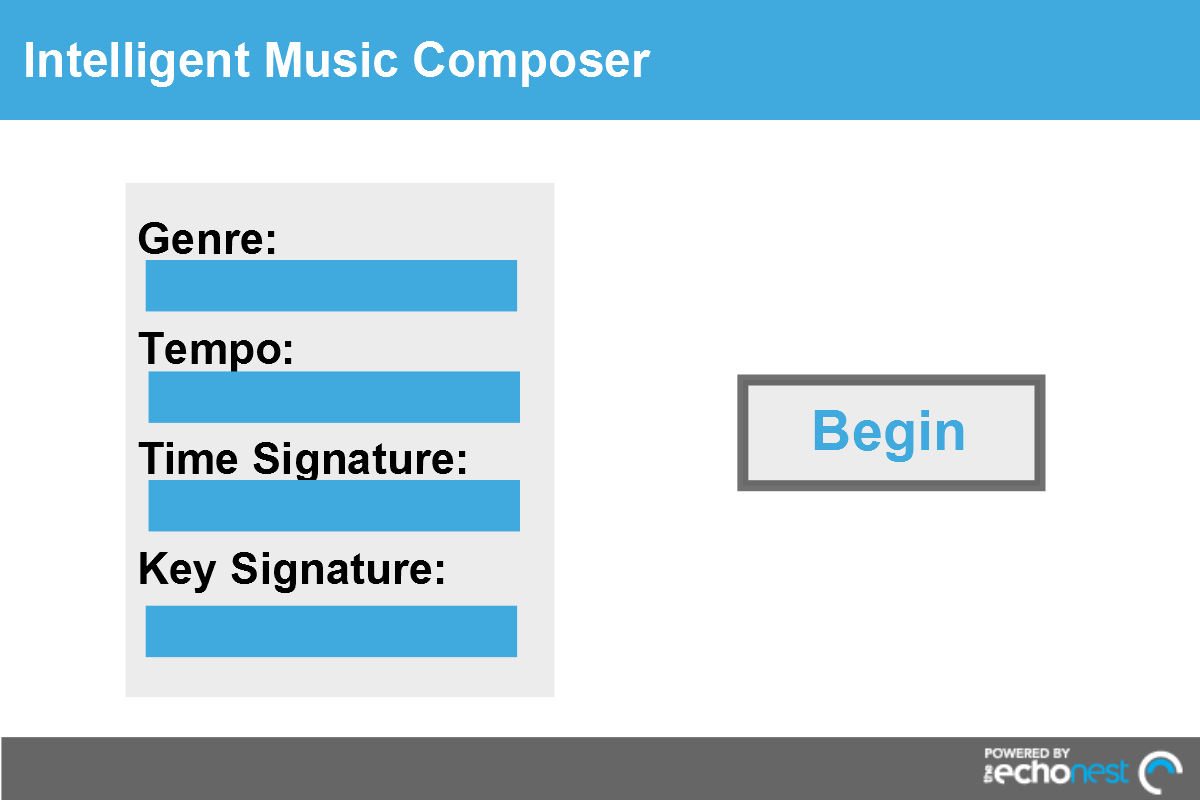
\includegraphics[width=10cm]{begin.png}}
\end{figure}

\begin{figure}[H]
\centerline{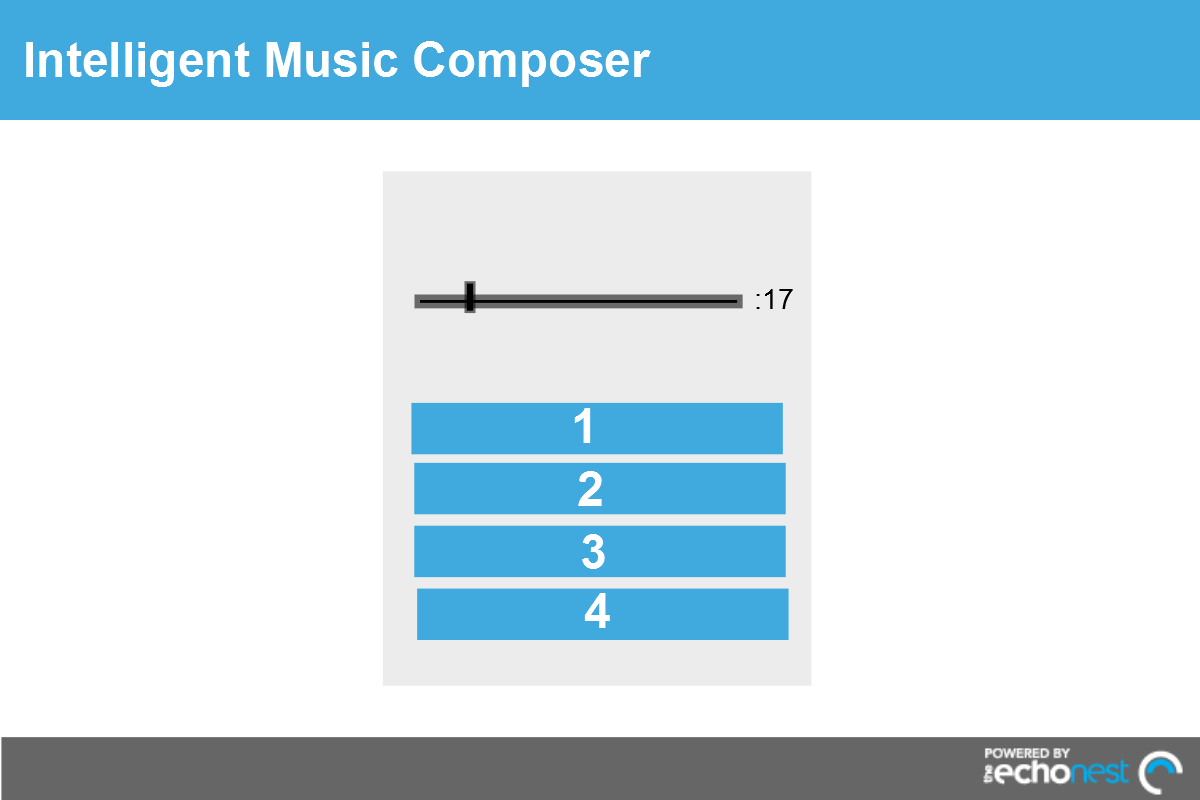
\includegraphics[width=10cm]{pref.png}}
\end{figure}

\begin{figure}[H]
\centerline{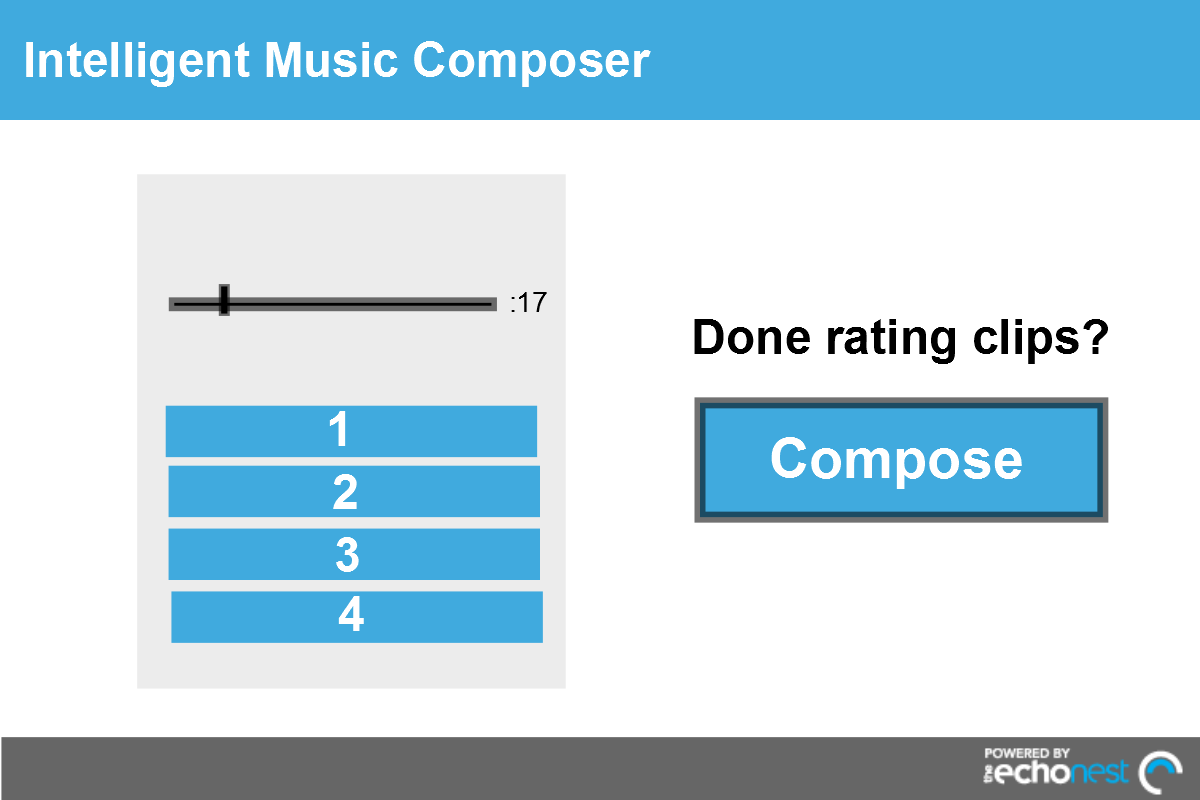
\includegraphics[width=10cm]{compose.png}}
\end{figure}

\section{Testing and Evaluation}
The testing is currently all manual. Each of the developers is responsible for testing all of their
components to make sure that they work properly, but the present focus of the project is the 
implementation of all required features. Once all of the desired features are implemented, a
more thorough testing procedure will be implemented to ensure the music generator works as designed.

\section{Project Progress}
\subsection{The Echo Nest Interface}
The Echo Nest interface is completely finished.  It is capabale of making a call to the Echo Nest's API using the 
user input and returning a list of song IDs, which the learning agent can utilize when it gathers user preferences
in the music clip rating portion of the application.

\subsection{Learning Agent}
<<<<<<< HEAD
Given the changes that have been made to the plan for the learning agent, it is now behind where schedule.
It takes in song IDs from the EN interface, and gathers relevant information about the songs.
\\
\Large{TODO: Ross, please fill in what you have been doing with the HHMMs}
=======
The learning agent is largely finished at this point in time. It is capable of reading in a sequence
of notes, applying the Baum-Welch algorithm to the data, and adjusting the parameters of it's data
model to better fit that sequence of notes.\\
\\
The main issue that is preventing the learning agent from being totally complete is the difficulty
of getting GHMM to accept a sequence of objects to learn from. This problem is currently being
handled by passing GHMM a carefully constructed string that represents each note object from a 
sequence. This solution could potentially work be used for the rest of the project; it is just
uglier and somewhat more difficult to read that if note objects were passed around, rather than
their string representations.
>>>>>>> 764473f4f38c9c273c07147afa2c6f0b99e595ce

\subsection{Composition Agent}
The composition agent has not been started, and will be the primary focus of the next phase in development.

\subsection{User Interface}
<<<<<<< HEAD
\Large{TODO: Ross, please fill in what you have done with the UI}
=======
>>>>>>> 764473f4f38c9c273c07147afa2c6f0b99e595ce
A basic, but functional user interface has been created that takes in genre, tempo, key signature, and time
signature from the user and passes those parameters to the Echo Nest interface. The user is then redirected
to a page where she will provide ratings of songs that the learning agent can utilize in its learning.

\section{Discussion}
<<<<<<< HEAD
Given that the project was called unoriginal, and uninnovative during it's last review, large changes have been
 made to the learning model that will be used. \Large{TODO: Ross, please fill the some basics about HHMMs}
=======
As previously discussed, the project is on pace to be completed by the end of the semester. There
have been various minor issues, but workarounds have been found for all of them, and as such, no
major changes have been made to the scope of the project.
>>>>>>> 764473f4f38c9c273c07147afa2c6f0b99e595ce

\newpage

\section{Appendices}
\subsection{Database Design}
As there is not a large quantity of data to be saved for this project, there is no associated 
database.

\subsection{User Manual}
Given the incomplete nature of the project at this point, a user manual is not appropriate.

\subsection{Programmer Manual}
Given the incomplete nature of the project at this point, a programmer manual is not appropriate.

\newpage

\bibliography{References}
\bibliographystyle{plain}

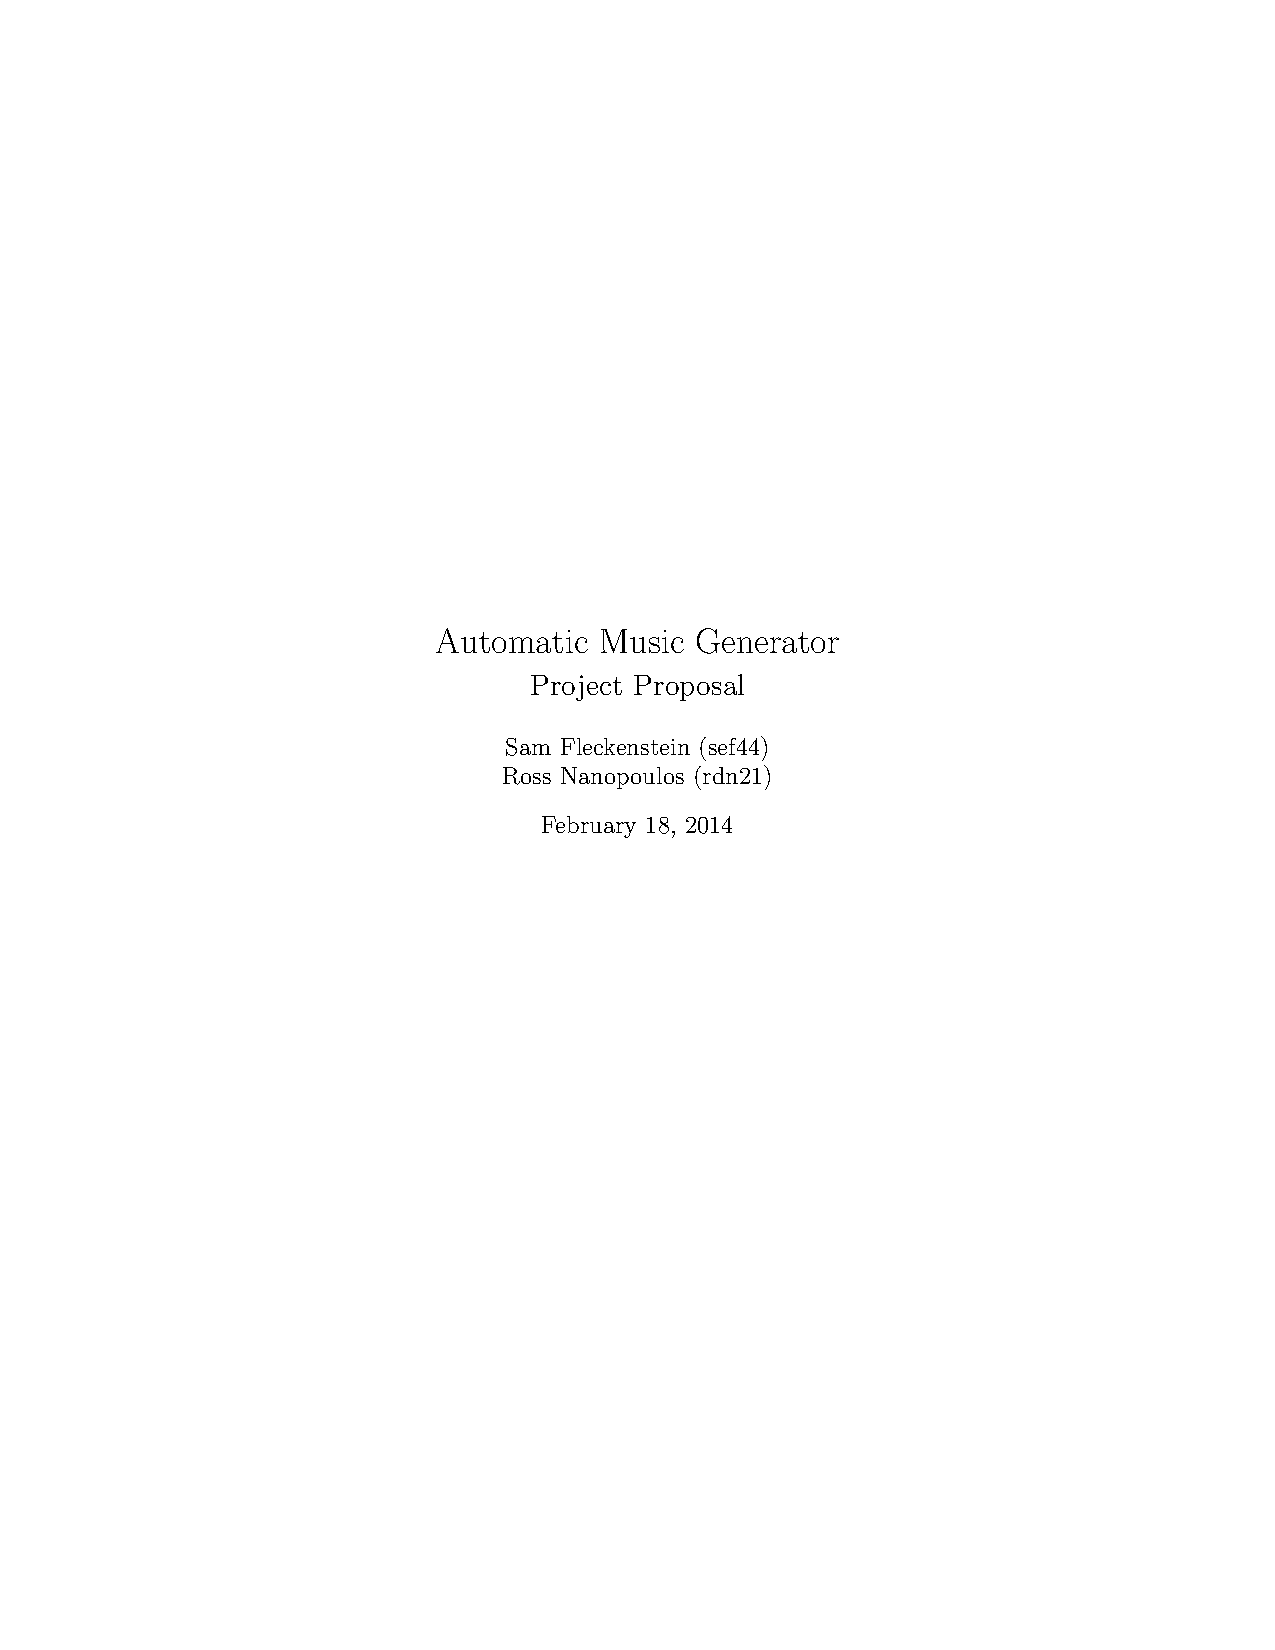
\includepdf[pages=-]{Proposal.pdf}

\end{document}
